% coding:utf-8

%FOSASTOC, a LaTeX-Code for a electrical summary of stochastic
%Copyright (C) 2013, Daniel Winz, Ervin Mazlagic

%This program is free software; you can redistribute it and/or
%modify it under the terms of the GNU General Public License
%as published by the Free Software Foundation; either version 2
%of the License, or (at your option) any later version.

%This program is distributed in the hope that it will be useful,
%but WITHOUT ANY WARRANTY; without even the implied warranty of
%MERCHANTABILITY or FITNESS FOR A PARTICULAR PURPOSE.  See the
%GNU General Public License for more details.
%----------------------------------------

\chapter{R Grundlagen}
\lstinline{R} ist eine multiparadigmatische Programmiersprache für 
Statistik und wird als Teil des GNU-Projektes entwickelt. Die 
Besonderheit von R liegt in der Implementation vieler Algorithmen
und Analysen der Statistik aber auch von vielseitigen Möglichkeiten 
des Plottens. Diese Stärken und die Tatsache, dass \lstinline{R} 
freie Software ist, haben es zu einem beliebten Tool in Wissenschaft
und Industrie gemacht.

\newpage

\setkeys{Gin}{width=1\textwidth}

\section*{Informationen finden}
Dieses Kapitel soll eine kurze Zusammenfassung der wichtigsten 
Funktionen in \lstinline{R} liefern. Möchte man spezifische und
detaillierte Informationen so kann man diese mittels \lstinline{help()}
erhalten. 

\section{Hilfe}
\lstinline{R} bietet für jede Funktion eine Art Manpage an. 
Diese kann in der Konsole mittels \lstinline{help(name-der-Funktion)}
aufgerufen werden. 

\begin{lstlisting}

\end{lstlisting}

\section{Vektoren \& Matrizen definieren}
\paragraph{Vektor mit Intervall 1 definieren}
\begin{Schunk}
\begin{Sinput}
> x <- 1:10; y <- 5:13
> x; y
\end{Sinput}
\begin{Soutput}
 [1]  1  2  3  4  5  6  7  8  9 10
\end{Soutput}
\begin{Soutput}
[1]  5  6  7  8  9 10 11 12 13
\end{Soutput}
\end{Schunk}

\paragraph{Vektor mit beliebigem festen Intevall definieren}
\begin{Schunk}
\begin{Sinput}
> x <- seq(from=1, to=10, by=2); y <- seq(1, 10, 2)
> x; y
\end{Sinput}
\begin{Soutput}
[1] 1 3 5 7 9
\end{Soutput}
\begin{Soutput}
[1] 1 3 5 7 9
\end{Soutput}
\end{Schunk}

\paragraph{Vektor manuell definieren}
\begin{Schunk}
\begin{Sinput}
> x <- c(77, 29, 12, 33, 4, 9, 809, -27)
> x
\end{Sinput}
\begin{Soutput}
[1]  77  29  12  33   4   9 809 -27
\end{Soutput}
\end{Schunk}

\paragraph{Matrix Spaltenweise definieren}
\begin{Schunk}
\begin{Sinput}
> a <- seq(1, 9, 1); m <- matrix(a, 3)
> m
\end{Sinput}
\begin{Soutput}
     [,1] [,2] [,3]
[1,]    1    4    7
[2,]    2    5    8
[3,]    3    6    9
\end{Soutput}
\end{Schunk}

\paragraph{Matrix Reihenweise definieren}
\begin{Schunk}
\begin{Sinput}
> a <- seq(1, 9, 1)
> m <- matrix(a, 3, byrow=TRUE)
> m
\end{Sinput}
\begin{Soutput}
     [,1] [,2] [,3]
[1,]    1    2    3
[2,]    4    5    6
[3,]    7    8    9
\end{Soutput}
\end{Schunk}

\section{Arithmetik}
\paragraph{Einfache Summen und Produkte}
\begin{Schunk}
\begin{Sinput}
> a=15; b=3
> a+b; a*b; a-b; a/b
\end{Sinput}
\begin{Soutput}
[1] 18
\end{Soutput}
\begin{Soutput}
[1] 45
\end{Soutput}
\begin{Soutput}
[1] 12
\end{Soutput}
\begin{Soutput}
[1] 5
\end{Soutput}
\end{Schunk}

\paragraph{Operationen auf Vektoren}
\begin{Schunk}
\begin{Sinput}
> a <- 1:10; b <- 2
> c <- b*a
> a
\end{Sinput}
\begin{Soutput}
 [1]  1  2  3  4  5  6  7  8  9 10
\end{Soutput}
\begin{Sinput}
> c
\end{Sinput}
\begin{Soutput}
 [1]  2  4  6  8 10 12 14 16 18 20
\end{Soutput}
\end{Schunk}

\paragraph{Operationen auf Matrizen}
\begin{Schunk}
\begin{Sinput}
> a <- seq(1, 9, 1); b <- 2
> m <- matrix(a, 3); n <- m*b
> m
\end{Sinput}
\begin{Soutput}
     [,1] [,2] [,3]
[1,]    1    4    7
[2,]    2    5    8
[3,]    3    6    9
\end{Soutput}
\begin{Sinput}
> n
\end{Sinput}
\begin{Soutput}
     [,1] [,2] [,3]
[1,]    2    8   14
[2,]    4   10   16
[3,]    6   12   18
\end{Soutput}
\end{Schunk}

\section{Spezielle Berechnungen}

\paragraph{Binomialkoeffizient}
\begin{Schunk}
\begin{Sinput}
> choose(7,2)
\end{Sinput}
\begin{Soutput}
[1] 21
\end{Soutput}
\end{Schunk}

\paragraph{Fakultät}
\begin{Schunk}
\begin{Sinput}
> factorial(5)
\end{Sinput}
\begin{Soutput}
[1] 120
\end{Soutput}
\end{Schunk}

\section{Plots}\label{sec:plots}

\subsection{Gewöhnlicher Plot}
Um einen gewöhnlichen Plot zu erstellen kann \lstinline{plot()}
verwendet werden. 

\begin{Schunk}
\begin{Sinput}
> x <- c(1:20)
> y <- (runif(n=20))
> plot(x, y)
\end{Sinput}
\end{Schunk}

\subsubsection{Linien plotten}
Möchte man einen Plot ergänzen mit Linien kann nach \lstinline{plot()}
noch \lstinline{abline()} benutzt werden.

\begin{Schunk}
\begin{Sinput}
> x <- c(1:20)
> y <- (runif(n=20))
> plot(x, y)
> abline(h=mean(y))
\end{Sinput}
\end{Schunk}

\subsubsection{Segmente plotten}
Möchte man beispielsweise die Abweichung von Daten und Mittelwert
zeigen, kann \lstinline{segments()} benutzt werden. Dieses ist in der
Lage mehrere Liniensegmente zu einem Plot hinzuzufügen.

\begin{Schunk}
\begin{Sinput}
> x <- c(1:20)
> y <- (runif(n=20))
> plot(x, y)
> abline(h=mean(y))
> segments(x0=x, y0=mean(y), x1=x, y1=y)
\end{Sinput}
\end{Schunk}

\subsubsection{Flächen plotten}
Möchte man Rechtecke oder Flächen in einen Plot einfügen so kann man 
\lstinline{rect()} benutzen. Im folgenden ein Beispiel zur Darstellung
der Varianz.

\begin{Schunk}
\begin{Sinput}
> x <- c(1:20)
> y <- (runif(n=20, min=3, max=7))
> plot(x, y, ylim=c(0, 10))
> abline(h=mean(y))
> diff <- sqrt((y-mean(y))^2)
> rect(xleft=x, xright=(x+diff), ybottom=mean(y), ytop=y, col='gray')
\end{Sinput}
\end{Schunk}

\begin{figure}[h!]
\centering
\begin{subfigure}[b]{0.48\textwidth}
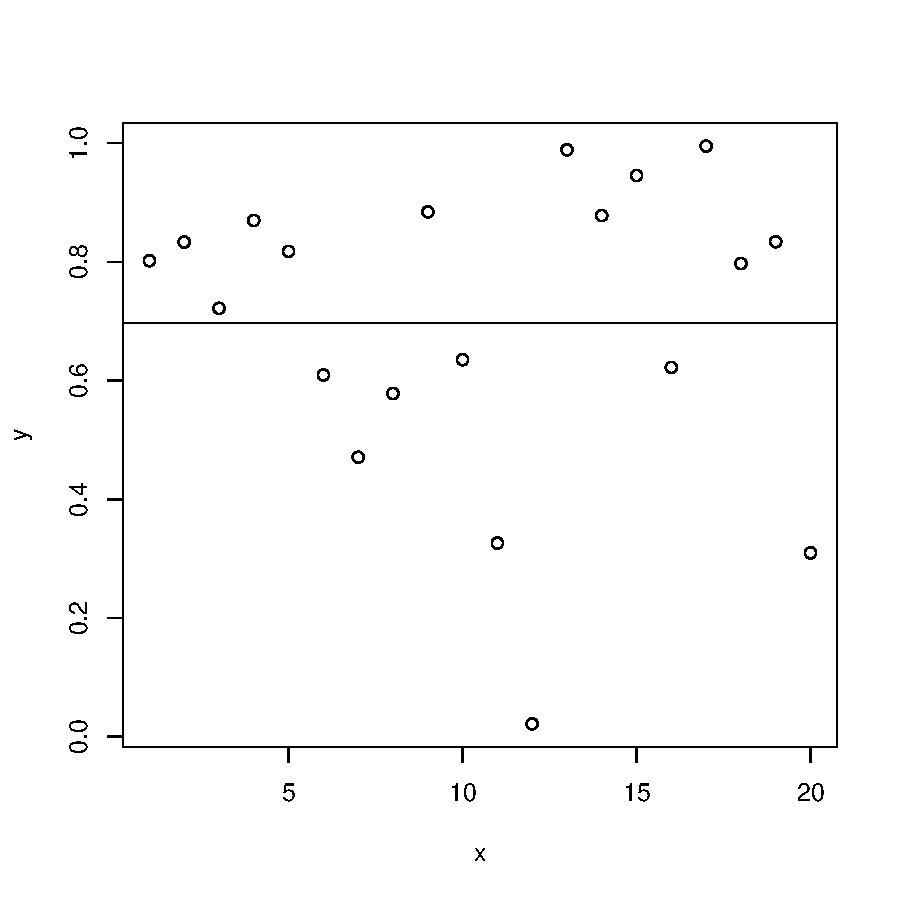
\includegraphics{r-cmd-015}
\caption{Gewöhnlicher Plot mit \lstinline{plot()}}
\end{subfigure}
\begin{subfigure}[b]{0.48\textwidth}
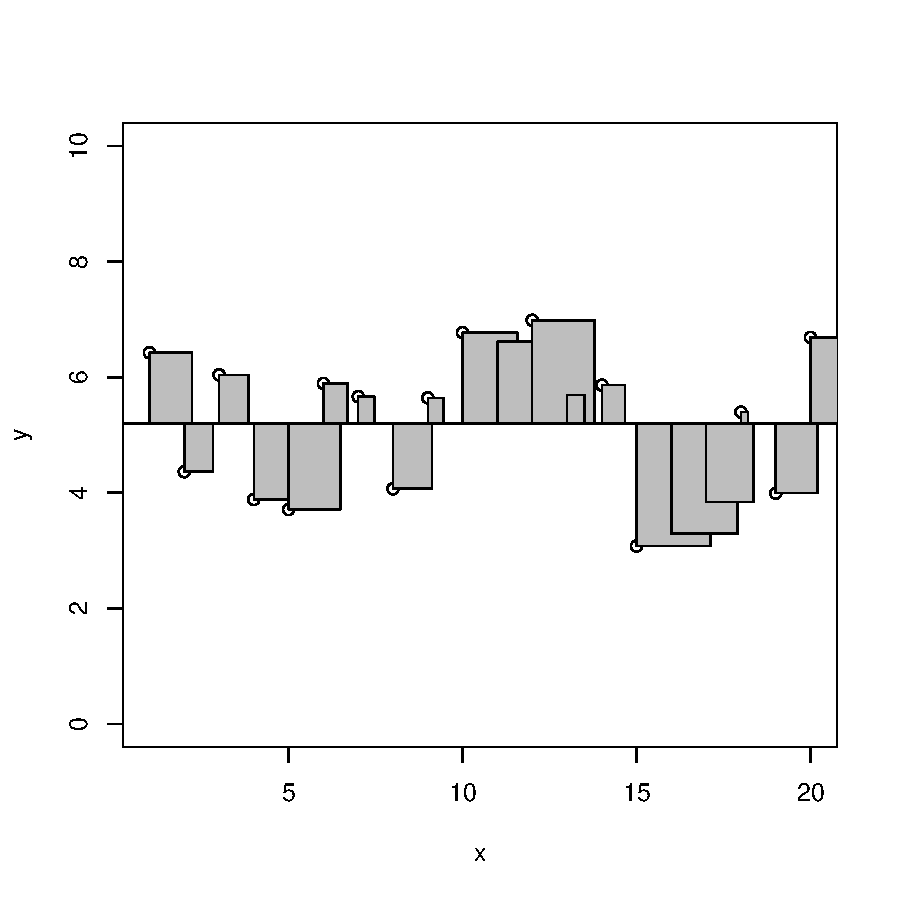
\includegraphics{r-cmd-016}
\caption{Linie mit \lstinline{abline()}}
\end{subfigure}

\begin{subfigure}[b]{0.48\textwidth}
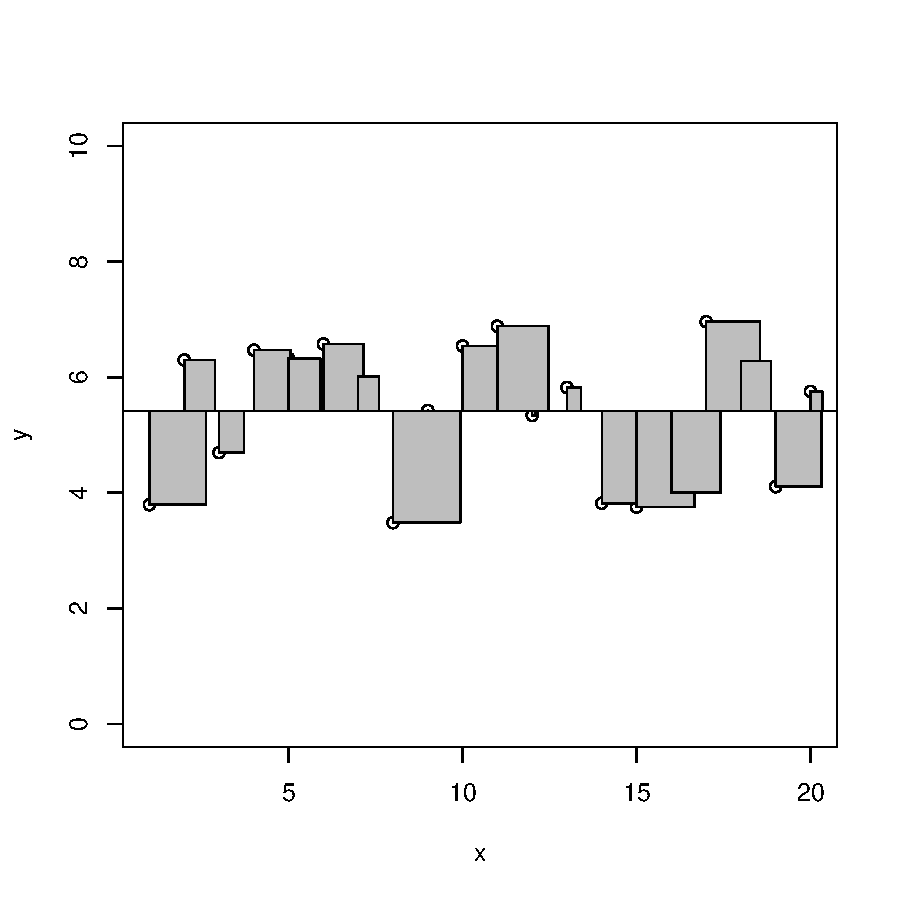
\includegraphics{r-cmd-017}
\caption{Segmente mit \lstinline{segments()}}
\end{subfigure}
\begin{subfigure}[b]{0.48\textwidth}
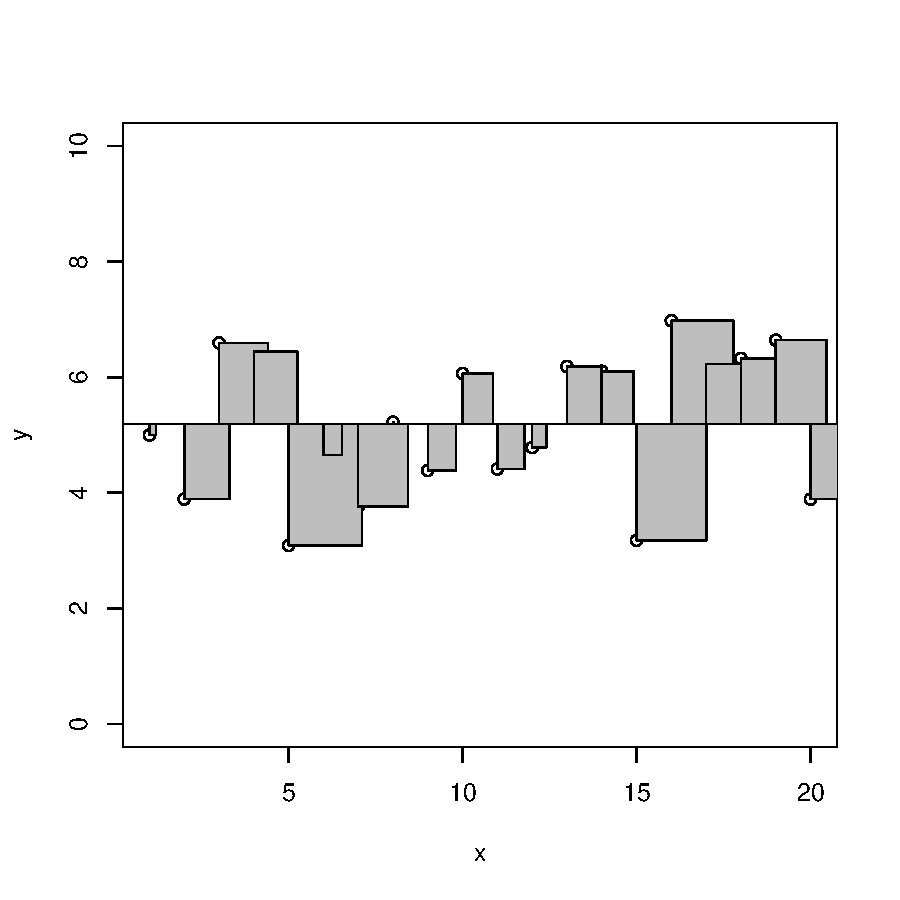
\includegraphics{r-cmd-018}
\caption{Flächen mit \lstinline{rect()}}
\end{subfigure}

\end{figure}

\clearpage

\subsection{Boxplot}
Ein Boxplot zeigt sehr viele Informationen zur Statistik einer 
Datenreihe in einem Plot auf. Insbesondere sind dies
\begin{itemize}
	\item extrem \emph{grosse} Beobachtungen
	\item die grösste \emph{normale} Beobachtung
	\item oberes Quartil ($75$\% Quantil)
	\item Median ($50$\% Quantil)
	\item unteres Quartil ($25$\% Quantil)
	\item die kleinste \emph{normale} Beobachtung
	\item extrem \emph{kleine} Beobachtungen
\end{itemize}
Die Abbildung \ref{fig:boxplot} zeigt einen Boxplot welches alle
oben genannten Merkmale gut sichtbat enthält.

\begin{figure}[h!]
	\centering
	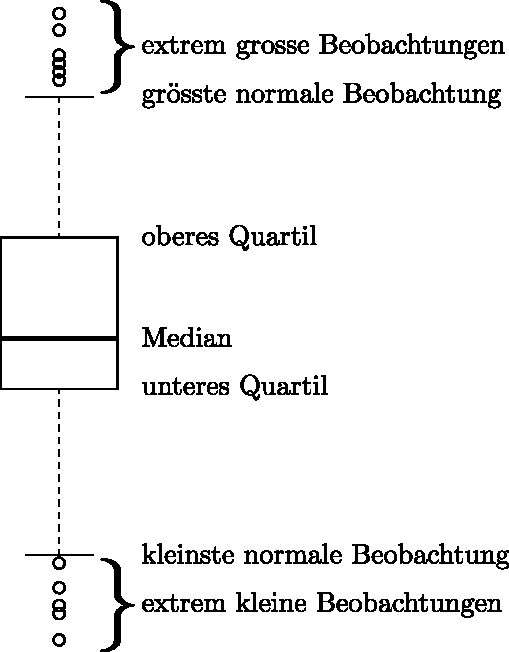
\includegraphics[width=0.5\textwidth]{boxplot.pdf}
	\caption{Analyse eines Boxplots}
	\label{fig:boxplot}
\end{figure}

\noindent
Mit solch einem Plot lässt sich die Verteilung einer Datenreihe sehr
schnell graphisch erfassen ohne dabei zu rechnen oder etwas 
interpretieren zu müssen. Jede Verteilung hat ihre spezielle 
Charakteristik die sich im Boxplot erkennen lässt.
\begin{itemize}
	\item Die uniforme Verteilung hat in etwa gleich grosse Bereiche
		der Quartile, ist somit symetrisch und geht über den 
		ganzen Bereich und hat somit keine Ausreisser 
		(Extremweerte).
	\item Die binomiale Verteilung hat enger beieinander liegende
		$25$\% Quantile und kann Ausreisser haben.
	\item Die normale Verteilung ist der binomialen sehr ähnlich.
	\item Exponentiale Verteilungen haben unsymetrische Quantile
		und grundsätzlich Ausreisser.
\end{itemize}





\begin{figure}[h!]
\centering
\begin{subfigure}[b]{0.48\textwidth}
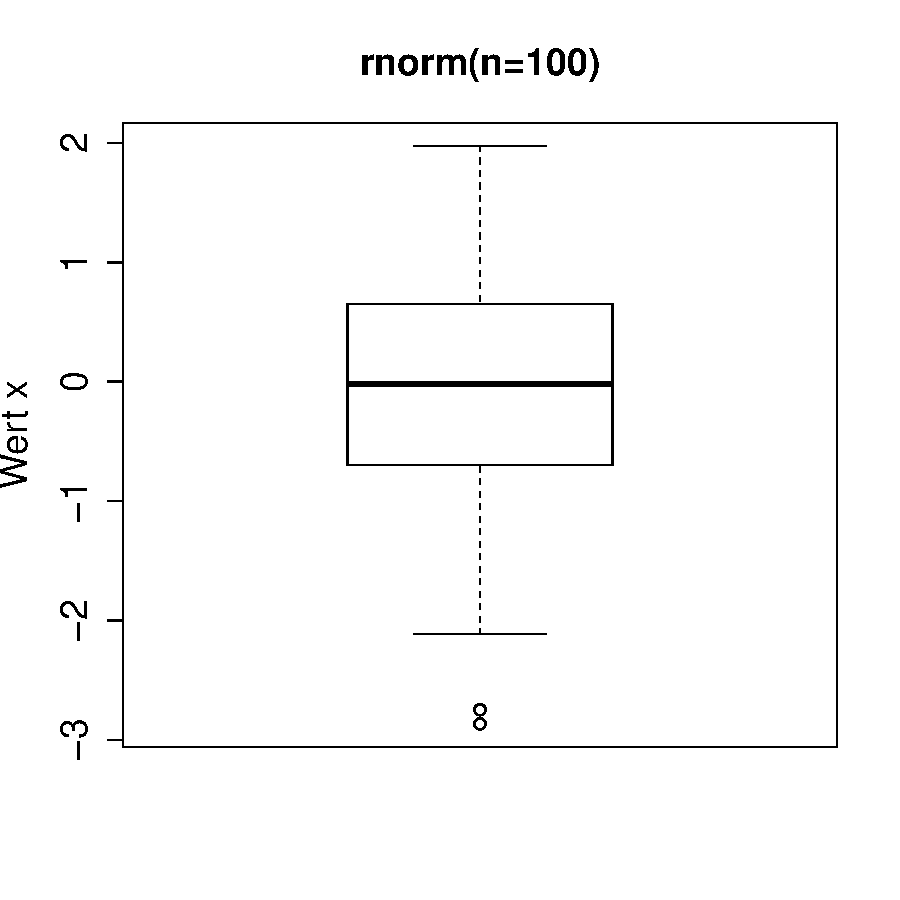
\includegraphics{r-cmd-023}
\caption{Uniforme Verteilung}
\end{subfigure}
\begin{subfigure}[b]{0.48\textwidth}
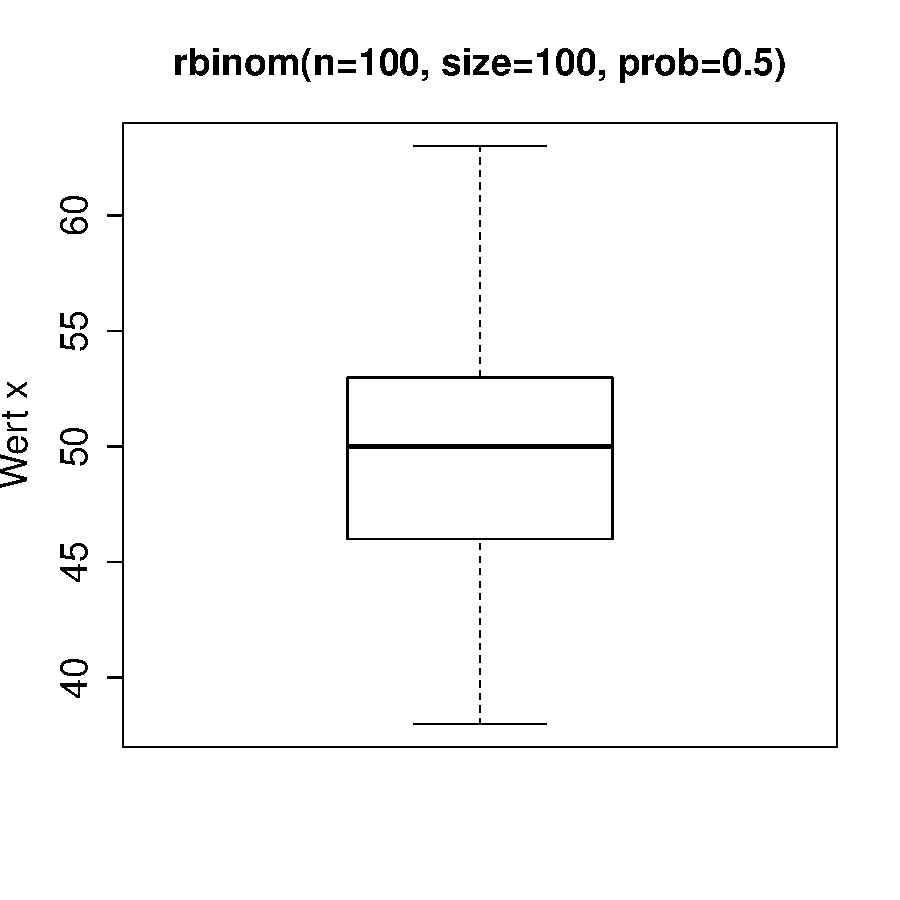
\includegraphics{r-cmd-024}
\caption{Binomiale Verteilung}
\end{subfigure}

\begin{subfigure}[b]{0.48\textwidth}
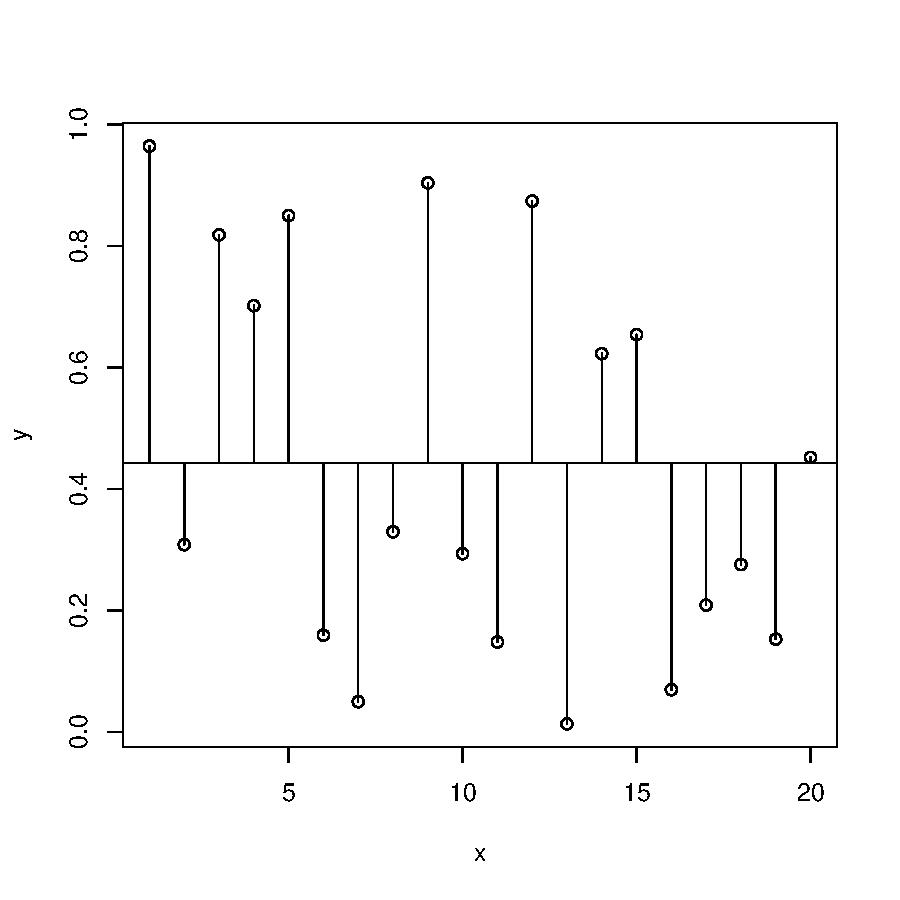
\includegraphics{r-cmd-025}
\caption{Normale Verteilung}
\end{subfigure}
\begin{subfigure}[b]{0.48\textwidth}
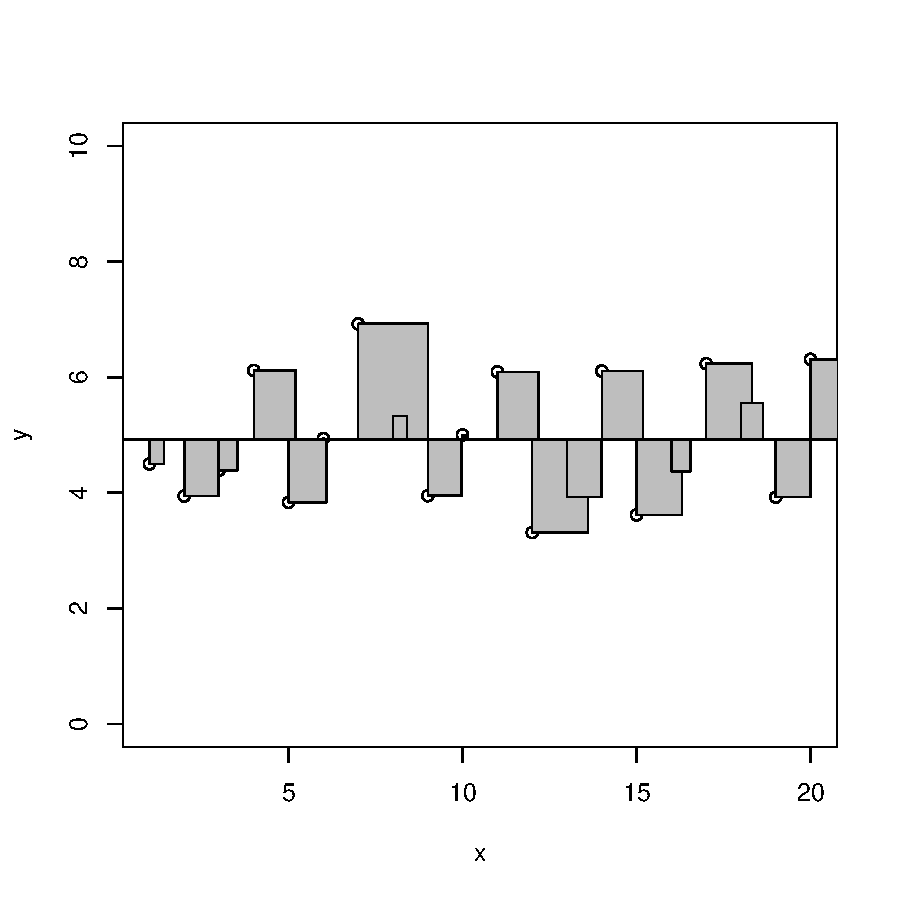
\includegraphics{r-cmd-026}
\caption{Exponential Verteilung}
\end{subfigure}
\caption{Boxplots verschiedener Verteilungen}
\end{figure}
